%% =====================================================================
%% Anschreiben (Cover Letter) — moderncv class, EIGENER kompakter Header
%% Auto-fillable base for the cover-letter automation.
%% See coverletter_automation.md for the workflow that fills it.
%%
%% Fields the automation replaces are marked:  % <<FILL: ...>>
%% Ships as a worked DE example (Loxone). Compile with MiKTeX:
%%   pdflatex anschreiben.tex
%%
%% NOTES:
%%  - moderncv already loads fontawesome6 — do NOT \usepackage fontawesome5.
%%    Use fontawesome6 names (\faRobot, \faLocationDot, \faDiagramProject, ...).
%%  - We bypass moderncv's \makelettertitle and typeset a compact, single-line
%%    contact header ourselves (moderncv's letter header stacks vertically).
%% =====================================================================

\documentclass[10pt,a4paper]{moderncv}   % <<FILL: 10pt>>
\moderncvstyle{banking}     % (nur für Fonts/Setup; Header ist unten custom)
\moderncvcolor{blue}

% ---- Encoding & language ------------------------------------------- % <<FILL: babel = ngerman|english>>
\usepackage[utf8]{inputenc}
\usepackage[T1]{fontenc}
\usepackage{lmodern}
\usepackage[ngerman]{babel}
\usepackage[scale=0.82]{geometry}

% ---- Extra packages (note, table) ----------------------------------
\usepackage{tcolorbox}
\usepackage{graphicx}
\usepackage{tabularx}
\usepackage{booktabs}
\usepackage{array}
% NOTE: do NOT load fontawesome5 — moderncv already provides fontawesome6.

% ---- Colors --------------------------------------------------------
\definecolor{accent}{HTML}{2C6E91}
\definecolor{ink}{HTML}{222222}
\definecolor{light}{HTML}{777777}
\definecolor{strongc}{HTML}{1F8A57}
\definecolor{partialc}{HTML}{C98A1B}
\definecolor{adjac}{HTML}{8A8A8A}
\definecolor{notebg}{HTML}{EAF2F6}

% ---- Strength badges (fontawesome6 names) --------------------------
\newcommand{\badge}[2]{\textcolor{#1}{\footnotesize\textbf{#2}}}
\newcommand{\strong}{\badge{strongc}{\faCircle\ stark}}            % <<FILL lang: strong|stark>>
\newcommand{\partialm}{\badge{partialc}{\faCircleHalfStroke\ teilw.}} % <<FILL lang: partial|teilw.>>
\newcommand{\adjacent}{\badge{adjac}{\faRegistered\ angrenz.}}

% Sender name (moderncv benötigt \name gesetzt; Header ist unten custom)
\name{Andreas}{Butry}

\begin{document}

% ---- Kompakter, einzeiliger Header (from profile.yaml: meta) -------
{\Huge\bfseries\color{accent}Andreas Butry}\\[1pt]
{\small\color{light}Funktionale Sicherheit, Software Qualität, Engineering-Prozesse \& KI-Innovation}\\[5pt]
{\color{accent}\rule{\linewidth}{1pt}}\\[4pt]
{\small\color{ink}%
\faLocationDot~Louise-Schroeder-Str.\ 2, 67551 Worms, Germany \;\textcolor{accent}{|}\;
\faPhone~+49\,179\,140\,90\,57 \;\textcolor{accent}{|}\;
\faEnvelope~\href{mailto:andreas.butry@gmail.com}{andreas.butry@gmail.com}\\[3pt]
\faGlobe~\href{https://andreasbutry.github.io/mypage/}{andreasbutry.github.io/mypage} \;\textcolor{accent}{|}\;
\faLinkedin~\href{https://www.linkedin.com/in/andreas-butry-23641530a}{LinkedIn-Profil}}

\bigskip

% ---- Empfänger & Datum   % <<FILL: recipient block>> ---------------
\begin{minipage}[t]{0.62\linewidth}
  Loxone Electronics GmbH\\
  Personalabteilung\\
  Schlossstraße 1\\
  4154 Kollerschlag, Österreich
\end{minipage}\hfill
\begin{minipage}[t]{0.33\linewidth}
  \raggedleft Worms, \today
\end{minipage}

\bigskip

% ---- Betreff   % <<FILL: role title>> ------------------------------
{\bfseries Bewerbung als \emph{Software Engineer (m/w/d)}}

\medskip

% ---- Transparenzhinweis --------------------------------------------
\begin{tcolorbox}[colback=notebg,colframe=accent,boxrule=0.8pt,arc=3pt,
                  left=8pt,right=8pt,top=5pt,bottom=5pt]
{\small\color{ink}\faRobot\enspace\textbf{Transparenzhinweis.}
Dieses Anschreiben wurde \textbf{in Teilen von einer KI-Automatisierung
geschrieben, die ich selbst entwickelt habe}: Sie liest die
Stellenausschreibung, erkennt deren Sprache, gleicht die Anforderungen mit
meiner Erfahrung ab ($\rightarrow$ \emph{Eignungstabelle auf Seite~2}) und
verfasst den Brief in der Sprache der Ausschreibung. Wie ich arbeite, sehen Sie
also bereits an diesem Dokument.}
\end{tcolorbox}

\medskip

Sehr geehrte Damen und Herren,

\medskip

% ---- Body: values-first opening   % <<FILL: values + matched evidence>>
% Ton: menschlich, keine Gedankenstriche "—"; erster Wort nach dem
% Anrede-Komma klein (außer Substantiv). Ein echter Satz zur Menschlichkeit.
gute Software entsteht für mich, wenn man \textbf{Komplexität strukturiert
herunterbricht}, \textbf{das große Ganze im Blick behält} und Qualität über einen
klaren \textbf{Verifikations-Mindset} absichert. Diese Haltung habe ich in über
acht Jahren sicherheitskritischer Entwicklung verinnerlicht, und genau sie möchte
ich bei \emph{Loxone} in vernetzte Produkte einbringen.

In meiner Laufbahn habe ich den gesamten System- und Software-Lebenszyklus
verantwortet: von Anforderungen und Architektur über Implementierung bis zur
Verifikation und Freigabe nach definierten Entwicklungsprozessen (z.\,B.
ISO~26262 und ASPICE). Aktuell entwickle ich bei
TES Electronics APIs für cloudbasierte Services und vernetzte
Home-Automation-Lösungen und baue Entwicklungsprozesse für KI-generierte
Software mit agentischen Workflows auf (stets mit menschlichem Review-Anteil,
Konzept \hyperlink{hitl}{\textbf{Human-in-the-Loop}} $\rightarrow$ Seite~2).

Neben der Technik ist mir ein menschlicher, respektvoller Umgang im Team wichtig,
gerade dann, wenn es einmal schwierig wird. Wie gut Ihre Anforderungen zu meiner
Erfahrung passen, habe ich auf Seite~2 in einer \textbf{Eignungstabelle}
zusammengestellt.

Über ein persönliches Gespräch würde ich mich sehr freuen.

% ---- Grußformel ----------------------------------------------------
\bigskip
Mit freundlichen Grüßen,\\[2.0em]
Andreas Butry

\medskip
{\small\color{light}Anlagen: Lebenslauf, Zeugnisse}

% ---- Werte-Liste (Seite 1) -----------------------------------------
\medskip
{\color{accent}\rule{\linewidth}{0.6pt}}\\[3pt]
{\small\bfseries\color{accent}Meine Engineering-Werte}\par\smallskip
{\small
\newcommand{\valitem}[3]{\par\noindent{\color{accent}#1}~\textbf{#2}: #3\par\vspace{1.5pt}}
\valitem{\faSitemap}{Komplexität herunterbrechen}{Strukturierte Arbeitspakete mit klaren Schnittstellen und Validierungspfaden.}
\valitem{\faDiagramProject}{Das große Ganze sehen}{Anforderungen, System, Prozesse und Stakeholder zusammen denken.}
\valitem{\faComments}{Klare Kommunikation}{Technische Themen verständlich machen und früh abstimmen.}
\valitem{\faCheckDouble}{Qualitätsfokus}{Traceability, Review-Disziplin und Verifikations-Mindset.}
\valitem{\faSeedling}{Kontinuierliches Lernen}{Methoden und Workflows verbessern, an Fehlern wachsen.}
\valitem{\faHandsHolding}{Menschlich \& empathisch}{Ruhig, respektvoll und lösungsorientiert.}
\valitem{\faShare}{Wissen teilen}{Dokumentation, Mentoring und offener Austausch.}
}

% =====================================================================
% APPENDIX (Seite 2): Eignungstabelle   % <<FILL: rows per JD requirement>>
% =====================================================================
\clearpage

{\Large\bfseries\color{accent}Eignungstabelle — Anforderungen \& Erfahrung}\\[2pt]
{\small\color{light}Automatisch aus der Ausschreibung abgeleitet und mit meinem
Profil abgeglichen. Legende:\;\strong\;\;\partialm\;\;\adjacent}

\medskip

\renewcommand{\arraystretch}{1.45}
\setlength{\tabcolsep}{10pt}
\begin{tabularx}{\linewidth}{@{}>{\raggedright\arraybackslash}p{0.28\linewidth} @{\hspace{16pt}} >{\raggedright\arraybackslash}X @{\hspace{16pt}} >{\centering\arraybackslash}p{0.13\linewidth}@{}}
\toprule
\textbf{Anforderung (Ausschreibung)} & \textbf{Beleg aus meiner Erfahrung} & \textbf{Match}\\
\midrule
Embedded-Softwareentwicklung & Embedded-/IoT-Software @ TES; sicherheitskritische Bremssteuergeräte @ Continental & \strong\\
APIs \& Cloud-Services & API-Design für cloudbasierte Services \& Home-Automation @ TES & \strong\\
Softwarequalität \& Prozesse & Entwicklung \& Prozessverantwortung nach ISO~26262 / ASPICE & \strong\\
KI-gestützte Entwicklung & Agentische Workflows, Prompt-/Context-Engineering, MCP (Claude Code) & \strong\\
\bottomrule
\end{tabularx}

% ---- Human-in-the-Loop-Grafik (unter der Tabelle, Seite 2) ---------
% <<FILL: Bildpfad relativ zum Brief. Template hier = coverletter_automation/;
%   generierte Briefe liegen in applications/<firma>_<rolle>/ → Pfad
%   ../../agents_in_sldc_final.png>>
\bigskip
\hypertarget{hitl}{}
{\Large\bfseries\color{accent}Konzept: Human-in-the-Loop}\\[2pt]
{\small\color{light}Aufbau meiner agentischen Workflows bei TES: jeder KI-Agent
mit menschlicher Prüfung und Freigabe vor dem nächsten Schritt.}

\smallskip

\begin{center}
  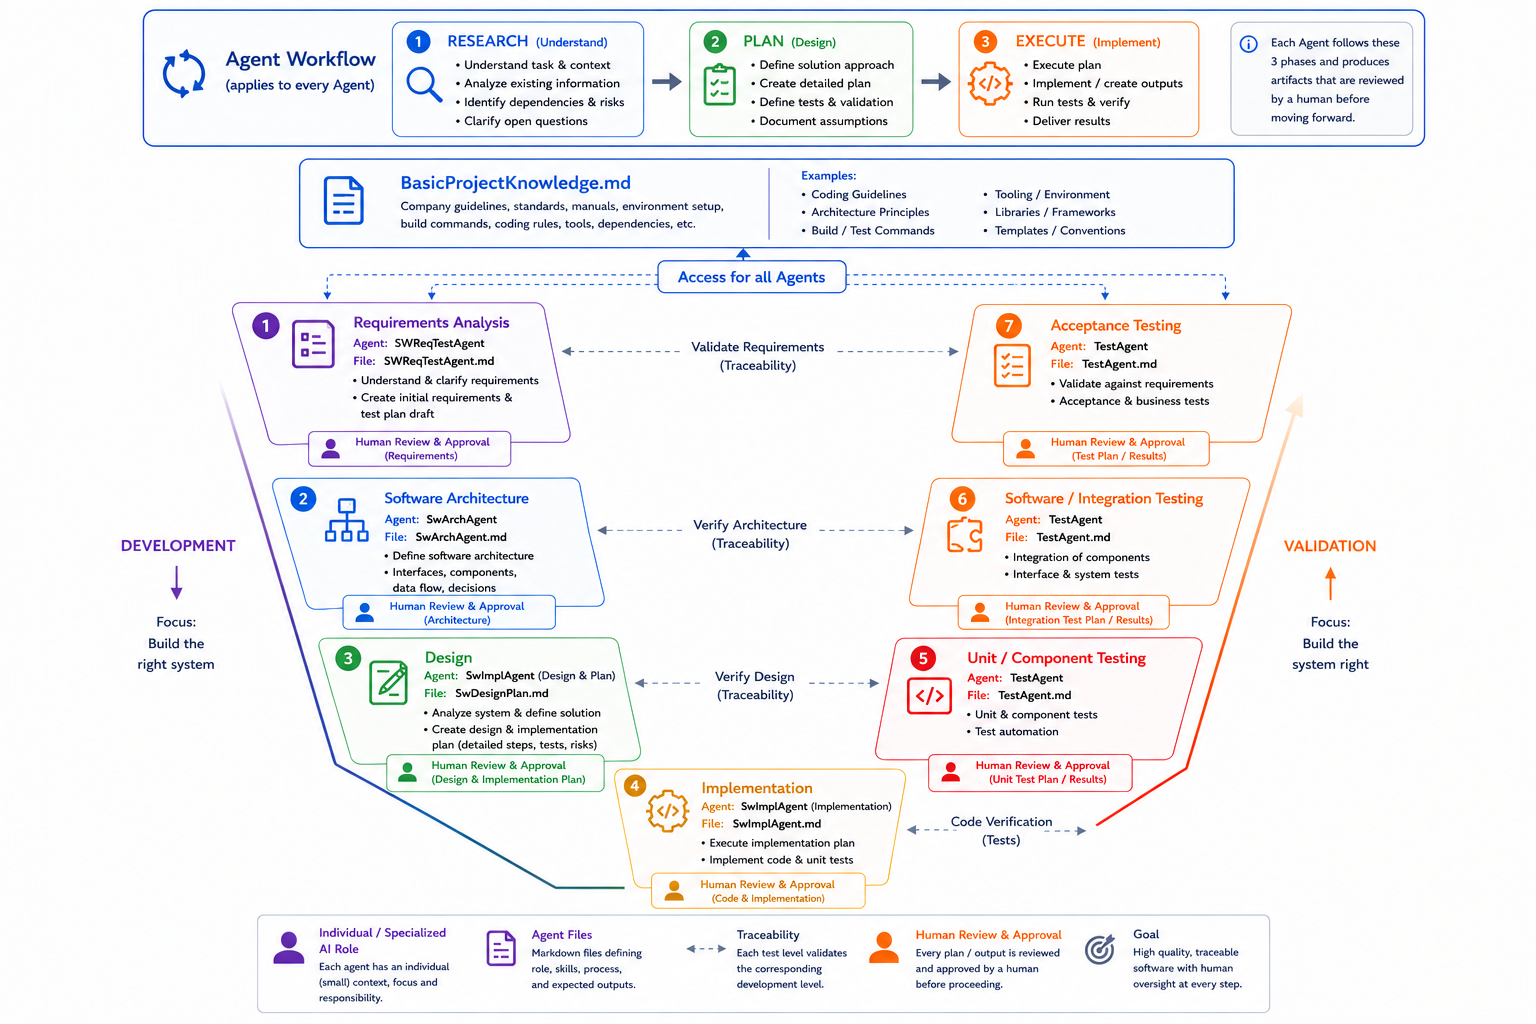
\includegraphics[width=0.9\linewidth]{agents_in_sldc_final.png}
\end{center}

\end{document}
